\documentclass[10pt,twocolumn,letterpaper]{article}



\usepackage{cvpr}
\usepackage{times}
\usepackage{epsfig}
\usepackage{graphicx}
\usepackage{amsmath}
\usepackage{amssymb}
\usepackage{subfigure}
\usepackage{color}
\usepackage{algorithm}
\usepackage{algorithmic}

\usepackage{amsmath,amssymb} % define this before the line numbering.
\usepackage{lineno}
\usepackage{color}
\usepackage{alltt}
\usepackage{verbatim}

% Include other packages here, before hyperref.

% If you comment hyperref and then uncomment it, you should delete
% egpaper.aux before re-running latex.  (Or just hit 'q' on the first latex
% run, let it finish, and you should be clear).
\usepackage[pagebackref=true,breaklinks=true,letterpaper=true,colorlinks,bookmarks=false]{hyperref}


% \cvprfinalcopy % *** Uncomment this line for the final submission

\def\cvprPaperID{745} % *** Enter the CVPR Paper ID here
\def\httilde{\mbox{\tt\raisebox{-.5ex}{\symbol{126}}}}

% Pages are numbered in submission mode, and unnumbered in camera-ready
\ifcvprfinal\pagestyle{empty}\fi
\begin{document}

%%%%%%%%% TITLE
\title{Common Fate Hough Transform for Concurrent Detection and Recognition}

\author{First Author\\
Institution1\\
Institution1 address\\
{\tt\small firstauthor@i1.org}
% For a paper whose authors are all at the same institution,
% omit the following lines up until the closing ``}''.
% Additional authors and addresses can be added with ``\and'',
% just like the second author.
% To save space, use either the email address or home page, not both
\and
Second Author\\
Institution2\\
First line of institution2 address\\
{\small\url{http://www.author.org/~second}}
}

\maketitle
% \thispagestyle{empty}

%%%%%%%%% ABSTRACT

\begin{abstract}
This paper proposes a method for concurrent detection and recognition of multiple multi-class objects by extending the probabilistic Hough transform to incorporate grouping results of the voting elements. In the method, each object part casts votes about the center and the class label of the object that generates itself. These object parts that will vote are firstly grouped by their motion patterns. The votes of each object part are assigned different priors according to the votes of the other object parts in the same motion group. The traceability of the Hough image formed by these votes is greatly enhanced. In such a manner, the proposed method meets the challenges of separating near objects and separating similar objects, while using a codebook trained from images with a clustered background. Experimental results are provided to show the merit in terms of detection and recognition accuracy.
\begin{comment}
The paper extends the . The extended Hough transform is employed to concurrently detect and recognize multiple multi-class objects. In the method, each object part casts votes about the center and the class label of the object that generates itself. These object parts that will vote are firstly grouped by their motion patterns. The votes of each object part are assigned different priors according to the votes of the other object parts in the same motion group. The traceability of the Hough image formed by these votes is greatly enhanced. In such a manner, the proposed method meets the challenges of separating near objects and separating similar objects, while using a codebook trained from images with a clustered background. Experimental results are provided to show the merit in terms of detection and recognition accuracy.
\end{comment}
\end{abstract}

%%%%%%%%% BODY TEXT
\section{Introduction}

The goal of the proposed method is to detect and recognize multiple multi-class objects on a given video frame. This is of importance for many applications, like surveillance and video analysis.

One reason, the generalized Hough transform~\cite{ac17} is favorable for detection and{\slash}or recognition, is its robustness to partial deformation, besides eigen window methods~\cite{ac18}, pictorial structures~\cite{ac2}, constellation models~\cite{ac3}, sliding window classifiers~\cite{ac4,ac1}, and branch-and-bound methods~\cite{ac1}. Object parts act as voting elements in the Hough transform based methods, in the form of keypoint descriptors~\cite{lb1}, image patches~\cite{ac6,ac7}, or image regions~\cite{ac8}. Each voting element votes for hypotheses that generate itself. The votes from different voting elements are added up to form a Hough image. The peaks of the Hough image are considered as detection hypotheses with the height of each peak as the confidence of the corresponding hypothesis. The simplicity of the learning procedure is another reason that the Hough transform based methods are attractive. An appearance codebook of object parts is built from a set of images on each of which the object center is annotated. Each code encodes the appearance and the offset to the object center of an object part. This offset acts as a Hough vote at run time, when object parts from the current image are matched against the codebook.

Besides the recent usage for various vision tasks~\cite{ac10,ac14,ac15,ac16}, the Hough transform based methods are extended for better detection performance. The implicit shape model~\cite{lb1,ac5} is extended  by notifying correspondences between the object parts and the hypotheses~\cite{ac9} for the detection of multiple near objects. The Hough transform is placed in a discriminative framework for object detection~\cite{ac10} in a way that the codes are assigned different weights by the co-occurrence frequency of their appearance and offset to the object center.

The proposed method not only detects multiple objects, but also recognizes each detected object. For recognition, the class label of each training image is annotated besides the object center. Then each code contains three aspects of information: the appearance, the offset to the object center, and the class label. The Hough image is formed by adding up votes with class labels, and the peaks of the Hough image are detection hypotheses with class labels. For each object, its location and class label are found from the hypotheses. However, for realistic scenarios with multiple multi-class objects, the Hough image formed in this manner is difficult to search over for concurrent detection and recognition.


One reason is that the object parts of the codebook are from multi-class objects, which even of the same class vary in poses. Thus the portion of the correct votes is low. For the traceability of the Hough image, the codebook needs to be very effective. So, the training images where objects appear as foreground need to have a very clean background. Otherwise, keypoints on the background act as noise and lead to false votes. The noisy votes make the portion of the correct votes even lower. Though computer graphics rendering provides a good source of clean-background images for the training of voting based methods~\cite{ac19}, in order to use real-world images with a clustered background, manual efforts are needed to mark the foreground, or a very large number of training images are needed to build the codebook, which harms efficiency.

Even if a very effective codebook is successfully built, the Hough image built upon a scene containing near objects and similar objects is still difficult to search over. This is due to two reasons: (1) votes casted by parts from two near objects make the peaks corresponding to different objects mixed up, and (2) different-class object parts are sometimes very similar, and this leads to tough decisions on the class label of the peaks.


To utilize the codebook built from training images with a clustered background and to meet the challenges of detecting near objects and recognizing similar objects, this paper proposes a concurrent detection and recognition method based on the common fate principle~\cite{ac13}. The principle is one of the four visual perception principles as theorized by gestalt psychologists. For humans, tokens moving coherently are perceptually grouped, and this provides an intuition to group the object parts (keypoint descriptors) that will vote by their motion patterns. The motion of each keypoint is represented by a trajectory generated by tracking the keypoint through frames.
The keypoints are then grouped using the pairwise similarities of their corresponding trajectories. Among the votes of each object part, those which are more {\lq\lq}agreeable{\rq\rq} by the votes of the other object parts in the same motion group are assigned higher priors. This results in correct votes being more likely to be assigned higher priors. These votes with different priors enhance the traceability of the Hough image for concurrent detection and recognition.

To the best of our knowledge, this is the first to incorporate motion information in the Hough transform based methods for concurrent detection and recognition. Additionally, the proposed method has several appealing properties:
\begin{itemize}
\item {The method realizes concurrent detection and recognition of multiple multi-class objects. The existence of three types of objects makes the task challenging: near objects, similar different-class objects, and multi-pose same-class objects.}
\item {Its ability to use a codebook trained by images with a clustered background.}
\item {The manner in which the grouping results by motion is integrated into the Hough transform is very general, and it can be used for incorporating other grouping results.}
\end{itemize}

The rest of the paper is organized as follows: The probabilistic Hough transform formulism for a concurrent detection and recognition problem is given in section 2. In Section 3 the formulism of the common fate Hough transform is given. The inference for concurrent detection and recognition is described in Section 4. Then experimental results are given in section 5, and section 6 concludes.


\section{Probabilistic Hough Transform}
This section describes how a Hough image for concurrent detection and recognition is formed from object parts observed on an image.

Let $\bf{e}$ denote an object part observed on the image. The appearance of $\bf{e}$ is matched against the codebook, and $\bf{e}$ activates $N$ best matched codes from the trained codebook. Each code contains the appearance, its offset to the object center, and the class label. According to the $N$ matched codes, $\bf{e}$ casts $N$ votes. Each vote $V_{\bf{e}}$ is about the object center that generates $\bf{e}$. The position of the object center casted by $V$ is denoted by ${\bf{x}}_V$, while the class label by $l_V$. Based on the $N$ votes of $\bf{e}$, the probability that a position $\tilde{\bf{x}}$ is the center of an object with class label $\tilde{l}$ is given by,

\begin{equation}p({\tilde{\bf{x}}},\tilde{l}|{\bf{e}}) = \sum\limits^N_{i=1} {p({\tilde{\bf{x}}},{\tilde{l}}|{V_{\bf{e}}^i}) p({V_{\bf{e}}^i}|{\bf{e}})}\:.
\label{eq1}
\end{equation}
Here $p({\tilde{\bf{x}}},{\tilde{l}}|{V_{\bf{e}}^i})$ is the likelihood of ${\tilde{\bf{x}}}$ being an object center of class ${\tilde{l}}$ based on $V_{\bf{e}}^i$. And $p({V_{\bf{e}}^i}|{\bf{e}})$ is the prior of ${V_{\bf{e}}^i}$, given ${\bf{e}}$.

The idea of the proposed method is that, the prior term, $p({V_{\bf{e}}^i}|{\bf{e}})$, is defined by the motion grouping results of all the object parts.

The likelihood term is defined as,

\begin{equation}
p(\tilde{\bf{x}},\tilde l|V)
= \left\{ \begin{array}{*{20}{c}}
   0   &\mbox{  if } {l_V} \ne \tilde{l} \mbox{ or } |\tilde{\bf{x}} - {\bf{x}}_V| > d   \\
   G(\tilde{\bf{x}};{{\bf{x}}_V},\sigma) &\mbox{otherwise}
\end{array} \right. \:.
\label{eq2}
\end{equation}
Here $G(\tilde{\bf{x}};{\bf{x}}_V,\sigma )$ is a Gaussian function that fixes the spacial gap between $\tilde{\bf{x}}$ and ${\bf{x}_V}$.

Let $M$ be the total number of object parts on the image, and assume the object parts are mutually independent.  Then by marginalizing over all the object parts, the probability of $\tilde{\bf{x}}$ being the center of a $\tilde{l}$-class object is given by,

\begin{equation}
\begin{aligned}
p({\tilde{\bf{x}}},\tilde{l}) &=\sum\limits^M_{j=1} p({\tilde{\bf{x}}},\tilde{l}|{\bf{e}}_j)p({\bf{e}}_j) \\
&{
\begin{aligned}
=\sum\limits^M_{j=1} \sum\limits^N_{i=1} {p({\tilde{\bf{x}}},{\tilde{l}}|{V_{{\bf{e}}_j}^i}) p({V_{\bf{e}}^i}|{\bf{e}}_j)p({\bf{e}}_j)} \:.
\end{aligned}
}
\end{aligned}
\label{eq3}
\end{equation}

Usually, a uniform prior is assumed for each object part, and $p({\bf{e}}_j)=\frac 1 M$. Then by considering $p({\tilde{\bf{x}}},\tilde{l})$ as the evaluation score of the Hough space $({\tilde{\bf{x}}},\tilde{l})$, the task of concurrent detection and recognition converts to finding and then validating the local maxima of the Hough image.

\section{Common Fate Hough Transform}
\begin{figure*}
\centering
\subfigure[]{
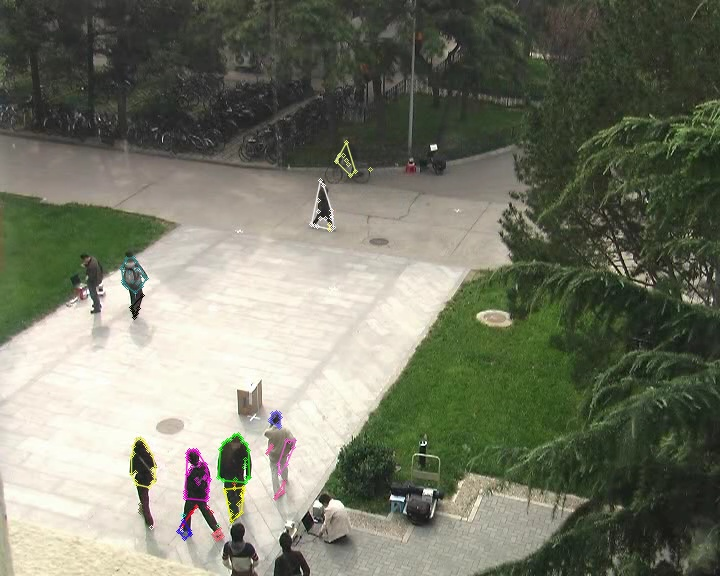
\includegraphics[width=0.22\textwidth,bb=0 0 720 576]{a56.jpg}
\label{fig:compa:a}}
\subfigure[]{
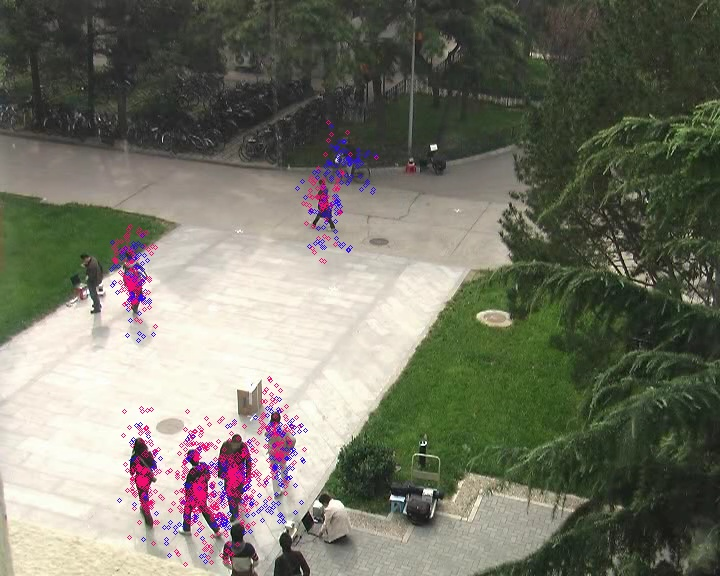
\includegraphics[width=0.22\textwidth,bb=0 0 720 576]{voteimg00056.jpg}
\label{fig:compa:b}}
\subfigure[]{
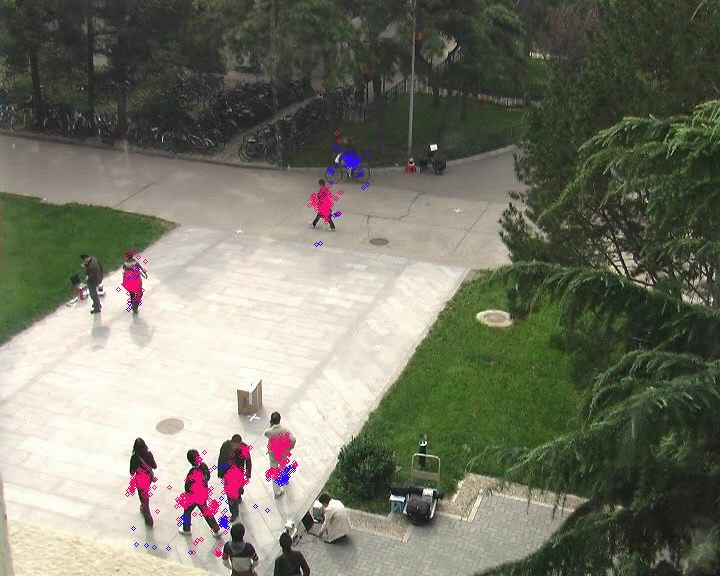
\includegraphics[width=0.22\textwidth,bb=0 0 720 576]{selectVimg00056_9.jpg}
\label{fig:compa:c}}
\subfigure[]{
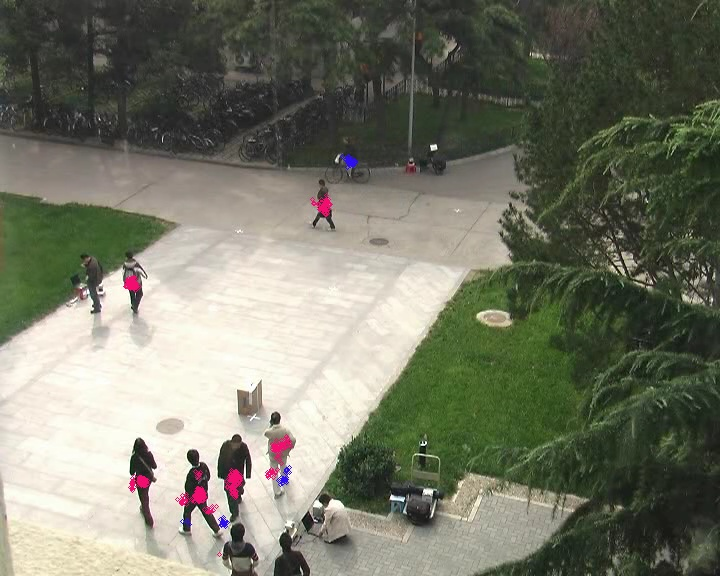
\includegraphics[width=0.22\textwidth,bb=0 0 720 576]{selectedvotesimg00056.jpg}
\label{fig:compa:c}}
\caption{Effect of the proposed prior. The motion grouping results are given in (a), and different motion groups are marked with different colors. The object centers voted according to the 7 best matched codes are given in (b). Red circles are centers of pedestrians while blue circles are centers of bicycle riders. The voted centers given in (c) are the voted centers of the 7 votes with the highest defined priors from 35 votes. The object centers in (d) are voted by votes with priors higher than 0.1.}
\label{fig:compa}
\end{figure*}
Since the codebook is trained by multi-class object parts and the training images have a clustered background, the best matched codes here cannot guarantee the traceability of the Hough image. This section describes how, by considering the motion grouping results of the object parts, different priors are assigned to the votes of each object part. 

Let $\gamma=\{\bf{g}\}$ denote the grouping results, where $\bf{g}$ is a group of object parts, i.e., ${{\bf{e}}_m}\in \bf{g}$ and ${{\bf{e}}_n}\in \bf{g}$. Those votes of ${\bf{e}_m}$ which are more {\lq\lq}agreeable{\rq\rq} by the votes of the other objects in $\bf{g}$ are assigned higher priors.

Towards this end, the relationship between the votes of $\bf{e}_m$ and the votes of $\bf{e}_n$ needs to be given in advance. This relationship is named support. The support from ${V_{{{\bf{e}}_n}}}$ to ${V_{{{\bf{e}}_m}}}$ is defined by that based on ${V_{{{\bf{e}}_n}}}$, the possibility ${V_{{{\bf{e}}_m}}}$'s voted center is correct, as,


\[
S({V_{{{\bf{e}}_n}}} \to {V_{{{\bf{e}}_m}}})  =  p({\bf{x}}_{V_{{{\bf{e}}_m}}},l_{V_{{{\bf{e}}_m}}}|{V_{{{\bf{e}}_n}}})\:,n \ne m\:.
\]
Here $p({\bf{x}}_{V_{{{\bf{e}}_m}}},l_{V_{{{\bf{e}}_m}}}|{V_{{{\bf{e}}_n}}})$ is defined in (\ref{eq2}). This measures the coherence of the two votes from different object parts.

Then, the support from ${{\bf{e}}_n}$ to ${V_{{{\bf{e}}_m}}}$ is defined by that based on ${{\bf{e}}_n}$, the possibility $V_{{{\bf{e}}_m}}$'s voted center is correct, as,

\[
\begin{aligned}
S({{{\bf{e}}_n} \to {V_{{{\bf{e}}_m}}}}) &= p({\bf{x}}_{V_{{{\bf{e}}_m}}},l_{V_{{{\bf{e}}_m}}}|{{{\bf{e}}_n}})\\
&=\sum\limits^N_{i=1} {p({\bf{x}}_{V_{{{\bf{e}}_m}}},l_{V_{{{\bf{e}}_m}}}|{V^i_{{{\bf{e}}_n}}})p(V^i_{{\bf{e}}_n}|{\bf{e}}_n)}\\
& {
=\sum\limits^N_{i=1} {S({{V^i_{{{\bf{e}}_n}}} \to {V_{{{\bf{e}}_m}}}})p(V^i_{{\bf{e}}_n}|{\bf{e}}_n)}\:,n \ne m\:.
}
\end{aligned}
\]

And the support from ${\bf{g}}$ to $V_{{\bf{e}}_m}$ is defined by the possibility that $V_{{\bf{e}}_m}$'s voted center is correct based on the votes of all the other object parts but its belonging object part in $\bf{g}$, as,
\[
\begin{aligned}
S({\bf{g}} \to V_{{\bf{e}}_m})
&= \sum\limits_{{{\bf{e}}_i} \in {\bf{g}}- \{ {{\bf{e}}_m} \} }{p({\bf{x}}_{V_{{{\bf{e}}_i}}},l_{V_{{{\bf{e}}_m}}}|{{{\bf{e}}_i}})p({{\bf{e}}_i})}\\
& =\frac 1 M  \sum\limits_{{{\bf{e}}_i} \in {\bf{g}}- \{ {{\bf{e}}_m} \}} {S({{{\bf{e}}_i} \to {V_{{{\bf{e}}_m}}}})} \:.
\end{aligned}
\]

Assuming all object parts in the same motion group are from the same object, which means motion grouping gives good results. The center position and the class label given by one vote shall be consistent with that given by the motion group.
Thus for a particular vote of ${\bf{e}}_m$, i.e., ${\tilde{V}}_{{\bf{e}}_m}$, a prior is assigned to it by considering its consistence with $\bf{g}$ and the consistence of ${\bf{e}}_m$'s other votes  with $\bf{g}$, as:
\begin{equation}
\begin{aligned}
{\color{blue}p(}&{\color{blue}{\tilde{V}}_{{\bf{e}}_m}|{\bf{e}}_m)}
= \frac
{S({\bf{g}} \to {{\tilde{V}}_{{\bf{e}}_m}}) + \frac{\Delta } N}
{\sum\limits^N_{i=1}{ S({\bf{g}} \to {V^i_{{{\bf{e}}_m}}})} + \Delta }\\
&
= \frac
{ \sum\limits_{{{\bf{e}}_j} \in {\bf{g}}- \{ {{\bf{e}}_m} \}} {S({{{\bf{e}}_j} \to {{\tilde{V}}_{{{\bf{e}}_m}}}})}  + \frac{M\Delta } N}
{\sum\limits^N_{i=1}{
\sum\limits_{{{\bf{e}}_j} \in {\bf{g}}-\{ {{\bf{e}}_m} \}} {S({{{\bf{e}}_j} \to {V^i_{{{\bf{e}}_m}}}})}
} + M\Delta }\\
&
\begin{aligned}
= \frac
{ \sum\limits_{{{\bf{e}}_j} \in {\bf{g}}- \{ {{\bf{e}}_m} \}} {
\sum\limits^N_{k=1} {S({{V^k_{{{\bf{e}}_j}}} \to {{\tilde{V}}_{{{\bf{e}}_m}}}})\color{blue}{p(V^k_{{\bf{e}}_j}|{\bf{e}}_j)}}
}  + \frac{M\Delta } N}
{\sum\limits^N_{i=1}{
\sum\limits_{{{\bf{e}}_j} \in {\bf{g}}- \{ {{\bf{e}}_m} \}} {
\sum\limits^N_{k=1} {S({{V^k_{{{\bf{e}}_j}}} \to {V^i_{{{\bf{e}}_m}}}})\color{blue}{p(V^k_{{\bf{e}}_j}|{\bf{e}}_j)}}
}
} + M\Delta }\:.
\end{aligned}
\end{aligned}
\label{eq4}
\end{equation}
Here, $\Delta$ is a small constant for preventing zeros. Notice, $p({\tilde{V}}_{{\bf{e}}_m}|{\bf{e}}_m)$ is defined using $p(V^k_{{\bf{e}}_j}|{\bf{e}}_j)$, the priors of the votes of the other object parts in ${\bf{g}}$. In order to give $p({\tilde{V}}_{{\bf{e}}_m}|{\bf{e}}_m)$, uniform priors are firstly assigned to the votes of each object part in ${\bf{g}}$, i.e., $p(V^k_{{\bf{e}}_j}|{\bf{e}}_j)=\frac{1}{N}$. Then new priors are calculated based on the uniformly assigned priors. The priors of votes to form the Hough image are priors converged in iterations.

The grouping results $\gamma=\{\bf{g}\}$, can be replaced by other grouping results of the voting elements. The proposed method uses motion to group the voting elements. The extended Hough transform with motion grouping results is called the common fate Hough transform. The voted centers voted by votes according to the best matched codes and the centers voted by votes with the highest priors are shown in Figure~\ref{fig:compa}. The centers voted by votes with highest priors defined here are more concentrated to the true object centers than the centers voted according to the best matched codes.

\subsection{Motion Grouping}
In order to group the object parts by their motion patterns. The object parts are tracked through frames before and after the current frame to generate trajectories. The object parts in this method are in the form of keypoint descriptors. The Harris Corner~\cite{harris} feature is chosen to represent the object part, while for appearance, the region covariance~\cite{regionc} of the image patch around the keypoint is used.

For each object part, a trajectory is generated by tracking its corresponding Harris Corner by the KLT tracker~\cite{ij2}.

To group the trajectories, pairwise similarities are firstly defined. Let $T_{{\bf{e}}_m}$ and $T_{{\bf{e}}_n}$ denote two trajectories corresponding to ${{\bf{e}}_m}$ and ${{\bf{e}}_n}$. The first similarity between two trajectories is defined as,
\[
{D_1}(T_{{\bf{e}}_m},T_{{\bf{e}}_n}) = \mathop {\max }\limits_{i=1...L} (Euclid({\bf{x}}^i_{T_{{\bf{e}}_m}},{\bf{x}}^i_{T_{{\bf{e}}_n}}))\:.
\]
Here, $Euclid$ calculates the Euclidean distance, $i$ is the frame index, and $L$ is the length of the overlapping part of the two trajectories.
To define the second similarity, the $i$th directional vector of $T$ is firstly defined as, ${\bf{d}}^i_T={\bf{x}}^{i+3}_{T}-{\bf{x}}^i_{T}$. Let ${\bf{a}}_i={\bf{d}}^i_{T_{{\bf{e}}_m}}$, ${\bf{b}}_i={\bf{d}}^i_{T_{{\bf{e}}_n}}$, $a_i=\frac{{{{\bf{a}}_i}\cdot{{\bf{b}}_i}}}{{{{\bf{a}}_i}\cdot{{\bf{a}}_i}}}$, and $b_i=\frac{{{{\bf{a}}_i}\cdot{{\bf{b}}_i}}}{{{{\bf{b}}_i}\cdot{{\bf{b}}_i}}}$. Then the second similarity is defined as,
\[
{D_2}(T_{{\bf{e}}_m},T_{{\bf{e}}_n})= \mathop {\max }\limits_{i=1...L-3} (\max (|{{\bf{a}}_i} - a_i {{\bf{a}}_i}|,|{{\bf{b}}_i} - b_i{{\bf{b}}_i}|))\:.
\]

To group the trajectories, the static points are firstly excluded. Inspired by \cite{my9}, a minimal spanning tree of the trajectories is built upon $D_1$, and split by cutting edges larger then a threshold, $D^1_{th}$. For each element of the splitting results, a minimal spanning tree is built upon $D_2$ and split by cutting the edges larger than a threshold, $D^2_{th}$. This hierarchical procedure ensures that trajectories in the same group have both small $D_1$ and $D_2$.

Each trajectory corresponds to an object part, and the grouping results of the trajectories correspond to grouping results of the object parts.
\subsection{Codebook}
For training, Harris corners are extracted from the training images with the object center and the class label annotated. In this method, region covariance is chosen to represent the appearance, which is defined as,
\[{\bf{r}} = \frac{1}{{K - 1}}\sum\limits_{i = 1}^K {({{\bf{z}}_i} - {\bf{\mu }}){{({{\bf{z}}_i} - {\bf{\mu }})}^T}} \;.\]
Here, $K$ is the number of pixels in the region, and ${{\bf{z}}_i}$ is a $7$-dimensional vector regarding the $(x,y)$ coordinate of the pixel, while ${\bf{\mu }}$ is the mean of ${{\bf{z}}_i}$.   And ${{\bf{z}}}(x,y)$ contains the RGB color of the pixel and intensity gradient of the pixel, as: $r(x,y)$, $g(x,y)$, $b(x,y)$, $|\frac {\partial I(x,y)} {\partial x}|$, $|\frac{\partial I(x,y)}{\partial y}|$, $|\frac{{\partial ^2}I(x,y)}{\partial {x^2}}|$, and $|\frac{{\partial ^2}I(x,y)}{\partial {y^2}}|$.

The appearance similarity between ${\bf{r}}_m$ and ${\bf{r}}_n$ is given by,
\[
\rho ({\bf{r}}_m,{\bf{r}}_n) = \sqrt {\sum\limits_{i = 1}^7 {{{\ln }^2}{\lambda _i}} }\;.
\]
Here, $\lambda _i$ is the generalized eigenvalue by solving the generalized eigenvalue problem, ${\lambda _i}{\bf{r}}_m{{\bf{u}}_i} = {\bf{r}}_n {{\bf{u}}_i},{{\bf{u}}_i} \ne {\bf{0}}$, with ${\bf{u}}_i$ the eigenvector.

A square image patch around each keypoint is used to represent the appearance of an object part. Six region covariances are generated for each image patch by using the pixels of the top-left, the top-right, the bottom-left, the bottom-right, the central, and all of the image patch. Then besides the offset and the class label, a code contains six region covariances. When an object part is matched against the codebook, the similarity between the image patch of the object part and a code is defined by the smallest similarity of the corresponding region covariances.


\section{Detection and Recognition}
After forming the Hough image, the detection and recognition hypotheses are validated. Let ${\bf{h}}=\{ H \}$ be the points in the Hough space which are evaluated by $p({\bf{x}}_{H},l_{H})$ and have $p({\bf{x}}_{H},l_{H})>0$.  Inspired by~\cite{ac9}, the hypotheses are validated by an optimizing procedure. Let $O$ be the number of the points in ${\bf{h}}$. let $u_i=1\mbox{ or } 0$ indicate $H_i$ being a true object center or not. The problem is:
\[
\arg \max\limits_{u_i} \prod\limits_{i = 1}^O { p^{u_i}({H_i})} \Longleftrightarrow\arg \max\limits_{u_i} \sum\limits_{i = 1}^O {{u_i}\ln (p({H_i})} )\:.
\]
Let $v_{ij}=1\mbox{ or } 0$ indicate $e_j$ belongs to $H_i$ or not, then
\[
\begin{aligned}
p(H_i)&=\sum\limits^M_{j=1} p({\bf{x}}_{H_i},l_{H_i}|{\bf{e}}_j)p({\bf{e}}_j)\\
&=\frac 1 M \sum\limits^M_{j=1} v_{ij} p({\bf{x}}_{H_i},l_{H_i}|{\bf{e}}_j)\:,
\end{aligned}
\]
and by assuming one object part belongs to and only belongs to one hypothesis, the problem is,
\[
\begin{aligned}
&\arg \max\limits_{u_i,v_{ij}} \sum\limits_{i = 1}^O {{u_i}\ln (\sum\limits^M_{j=1} v_{ij} p({\bf{x}}_{H_i},l_{H_i}|{\bf{e}}_j)} )\\
&
\begin{aligned}
    s.t.:\mbox{ }&u_i=0\mbox{ or }u_i=1,\forall\;i\\
    &v_{ij}=0\mbox{ or }v_{ij}=1,\forall\;i,\forall\;j\\
    &\sum\limits_{i = 1}^O {v_{ij}}=1,\forall\;j\\
    &\sum\limits_{j = 1}^M {v_{ij}}<=u_i,\forall\;i\:.
\end{aligned}
\end{aligned}
\]


Following~\cite{ac9}, the optimal result for the problem is inferred by greedy maximization. As described in Algorithm~\ref{alg:gm}, the largest local maximum of all the local maxima is chosen to be the center of a true object and then the object parts belonging to the chosen object center are excluded from the object part set. A new Hough image where new objects are found is formed using the remaining object parts. This procedure ends when the object part set is empty or the confidence of the chosen object is lower than a threshold.
\begin{algorithm}[h]

    \caption{Greedy Maximization}
    \label{alg:gm}
     Let $\varepsilon$ be the set of object parts, $p_{th}$ be the low confidence threshold to accept detection responses, and $\hat{\bf{h}}$ be the local maxima of $\bf{h}$

    \begin{algorithmic}[1]




        \WHILE {$\varepsilon \ne \emptyset$}

            \STATE Form $\bf{h}$ with $\varepsilon$\\

            \STATE Generate $\hat{\bf{h}}$ and select $H_i \in {\hat{\bf{h}}},$\\ $u_i=0 \mbox{ and }\forall {H^{'}} \in {\hat{\bf{h}}, p({\bf{x}}_{H_i},l_{H_i}) >= p({\bf{x}}_{H^{'}},l_{H^{'}}) } $
            \IF {$p({\bf{x}}_{H_i},l_{H_i}) >=p_{th}$}

                \STATE $u_i\leftarrow1$

                \FOR{${\bf{e}}_j\in \varepsilon$}

                    \IF{$\forall {H^{'}} \in {\hat{\bf{h}}}, p({\bf{x}}_{H_i},l_{H_i}|{\bf{e}}_j) >= p({\bf{x}}_{H^{'}},l_{H^{'}}|{\bf{e}}_j)$}

                    \STATE $v_{ij}\leftarrow1$

                    \STATE $\varepsilon\leftarrow \varepsilon -\{ {\bf{e}}_j \}$

                    \ENDIF

                \ENDFOR

            \ELSE

                \FOR {${\bf{e}}_j \in \varepsilon$}

                \STATE $v_{1j}\leftarrow1$

                \ENDFOR

                \STATE $\varepsilon\leftarrow \emptyset$

            \ENDIF

        \ENDWHILE
    \RETURN all $u_i,u_i=1$

    \end{algorithmic}

\end{algorithm}

\section{Experimental Results and Evaluation}
In the experiments, the enhancement of the Hough image's traceability by the method is verified in terms of detection accuracy and recognition accuracy. The method is firstly tested on the \emph{P-campus} dataset with~\cite{ac9} as benchmark, and then tested on a dataset of similar animals.
\subsection{ Campus Objects Detection and Recognition}

\textbf{Dataset} The \emph{P-campus} dataset contains two primary classes of foreground objects: pedestrians and bicycle riders. The frame size is 720$\times$576. Among all the 401 continuous frames, 633 different-class ground truth bounding boxes are annotated on 79 frames. In this dataset, pedestrians and bicycle riders have in common the upper human body, and pedestrians appear in front, back, and side views.

\textbf{Implementation Settings} For training, 52 images of bicycle riders and 171 images of pedestrians are randomly selected. Harris corners are generated on the image, and training image examples are given in Figure \ref{fig:train:a}. For appearance, six region covariances are generated for each keypoint using the 9$\times$9 image patch around it as shown in Figure \ref{fig:train:b}. The appearance, the offset to the image (object) center, and the label of the training image are encoded, and the code is inserted into a codebook. The final codebook contains 5502 codes.

\begin{figure}
\centering
\subfigure[]{
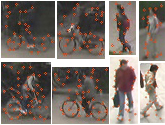
\includegraphics[width=0.23\textwidth,bb=0 0 165 125]{samples.jpg}
\label{fig:train:a}
}
\subfigure[]{
{
\begin{minipage}[b]{0.2\textwidth}
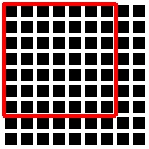
\includegraphics[width=0.32\textwidth,bb=0 0 149 149]{dst6.jpg}
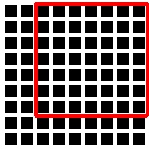
\includegraphics[width=0.32\textwidth,bb=0 0 149 149]{dst3.jpg}
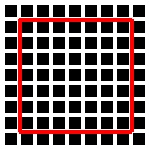
\includegraphics[width=0.32\textwidth,bb=0 0 149 149]{dst5.jpg}\\
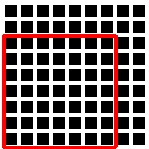
\includegraphics[width=0.32\textwidth,bb=0 0 149 149]{dst2.jpg}
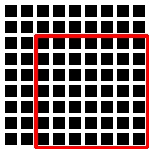
\includegraphics[width=0.32\textwidth,bb=0 0 149 149]{dst4.jpg}
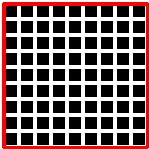
\includegraphics[width=0.32\textwidth,bb=0 0 149 149]{dst1.jpg}
\end{minipage}
}
\label{fig:train:b}
}
\caption{Examples of training images are given in (a). The red circles are the extracted Harris corners. Some keypoints fall on the background. The six rectangles in (b) mark the pixels of the 9$\times$9 image patch used for the six region covariances.}
\label{fig:train}
\end{figure}
\begin{figure*}
\centering
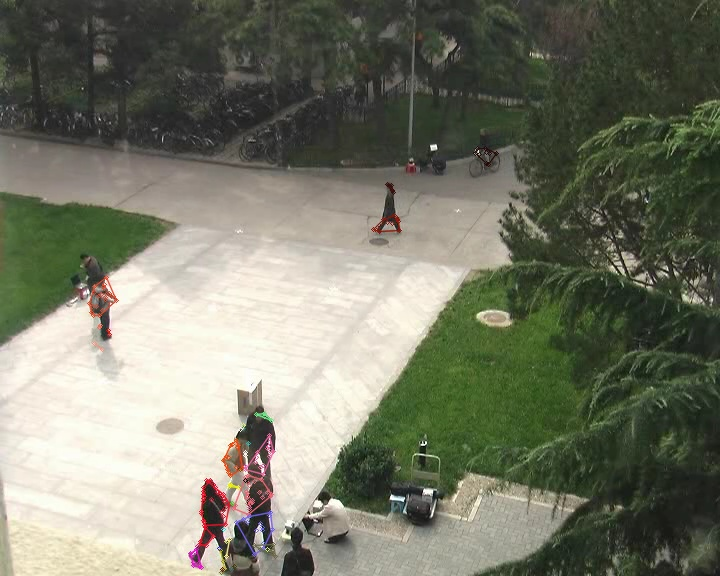
\includegraphics[width=0.23\textwidth,bb=0 0 720 576]{a16.jpg}
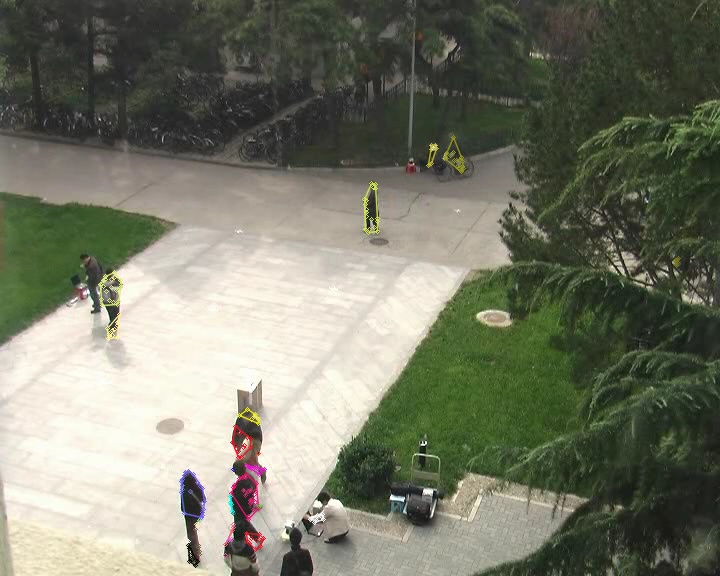
\includegraphics[width=0.23\textwidth,bb=0 0 720 576]{a26.jpg}
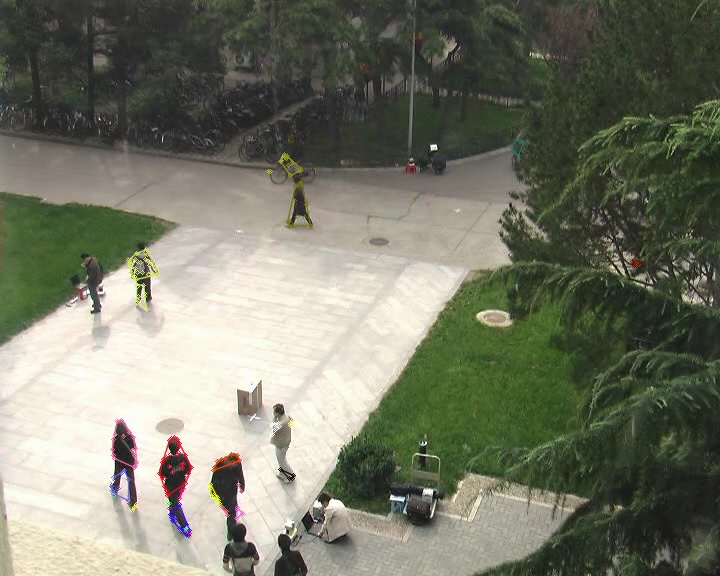
\includegraphics[width=0.23\textwidth,bb=0 0 720 576]{a71.jpg}
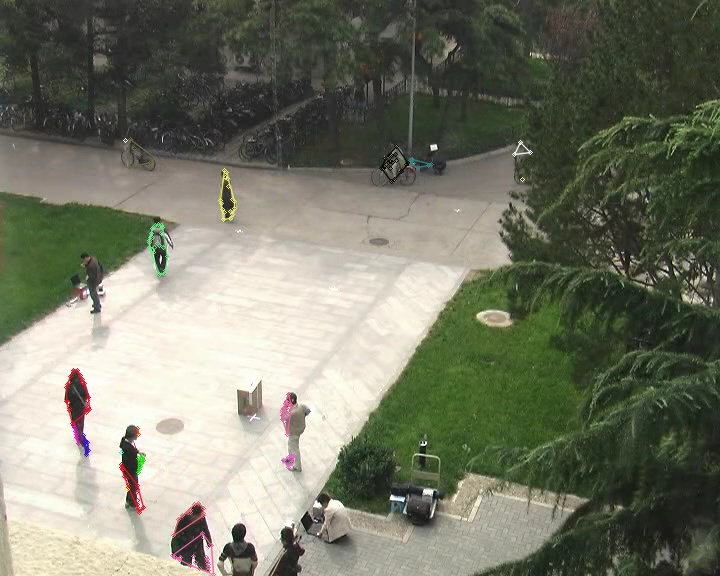
\includegraphics[width=0.23\textwidth,bb=0 0 720 576]{a116.jpg}
\caption{Motion grouping results.}
\label{fig:mgr}
\end{figure*}

For motion grouping, each keypoint is tracked through 10 frames before and through 10 frames after the current frame. The similarity of two 21-point trajectories is defined using only the overlapping part. To set the two thresholds for motion grouping, $D_1$ and $D_2$ are  measured for keypoint pairs of different objects. $D^1_{th}$ is set that it is larger than only 10\% of the measured $D_1$s, and so is $D^2_{th}$. By doing so, keypoints belonging to different objects are not likely to be grouped together. So, in one motion group, the keypoints are very likely to belong to the same object, as shown in Figure \ref{fig:mgr}.



\begin{figure*}
\centering
\subfigure[]{
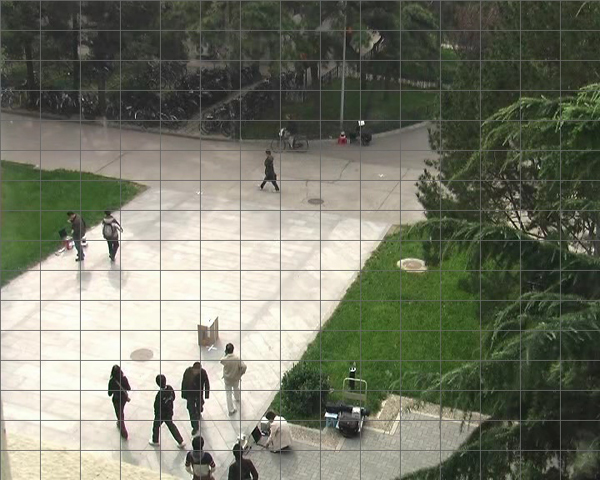
\includegraphics[width=0.22\textwidth,bb=0 0 600 480]{PEssR.jpg}}
\subfigure[]{
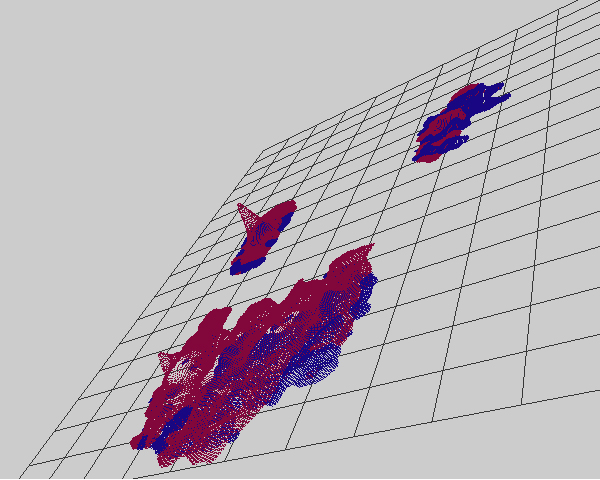
\includegraphics[width=0.22\textwidth,bb=0 0 600 480]{Untitled-6.jpg}}
\subfigure[]{
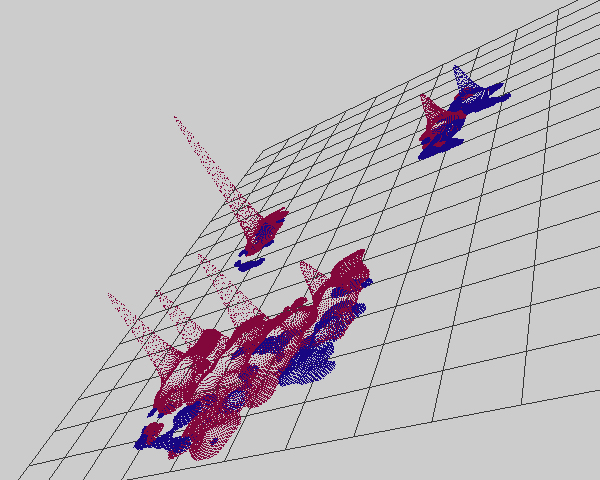
\includegraphics[width=0.22\textwidth,bb=0 0 600 480]{Untitled-5.jpg}}
\subfigure[]{
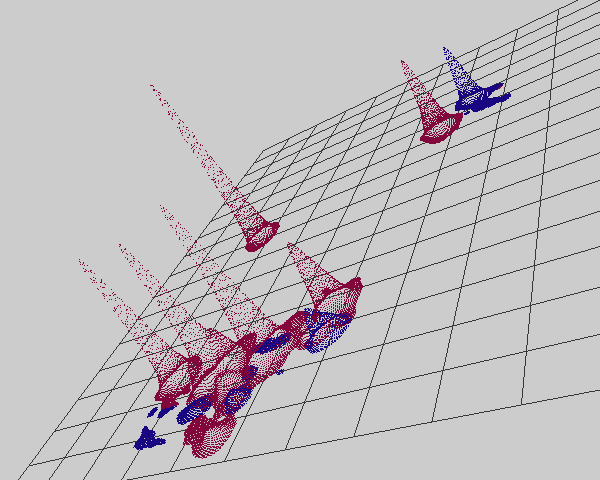
\includegraphics[width=0.22\textwidth,bb=0 0 600 480]{Untitled-4.jpg}}

\caption{Example Hough images. Grids in (b), (c), and (d) correspond to the grids on the image coordinate. Red indicates pedestrians, while blue indicates bicycle riders. Hough image of (b) is formed by votes with uniform priors, Hough image of (c) is formed by votes with priors after 5 iterations, and Hough image in (d) is formed with converged priors.}
\label{fig:Hough}
\end{figure*}

To form the Hough image, 35 best matched codes are chosen from the codebook for each object part. In (\ref{eq3}), $d$ and $\sigma$ need to be given. The precision-recall curves are based on $\sigma$, while $d$ is set to be 10. Here $\sigma$ is the most important parameter, while changing d from 5 to 16 only results in a 1\% difference in the detection rate. For Algorithm \ref{alg:gm}, $p_{th}$ is set to be 0, which means all local maxima found in Algorithm \ref{alg:gm} are accepted.

\textbf{Comparisons} For comparison, concurrent detection and recognition are done on the Hough images formed with and without motion grouping results. The same codebook and the same parameter settings are used for forming and searching over both Hough images. The votes of each object part are assigned uniform priors in the benchmark method, while priors defined in (\ref{eq4}) are assigned in the proposed method. Example Hough images are shown in Figure \ref{fig:Hough}. With the noisy codebook, peaks of different objects on the original Hough image not only mix up in position but also in class label.




\begin{figure}
\centering
\subfigure[]{
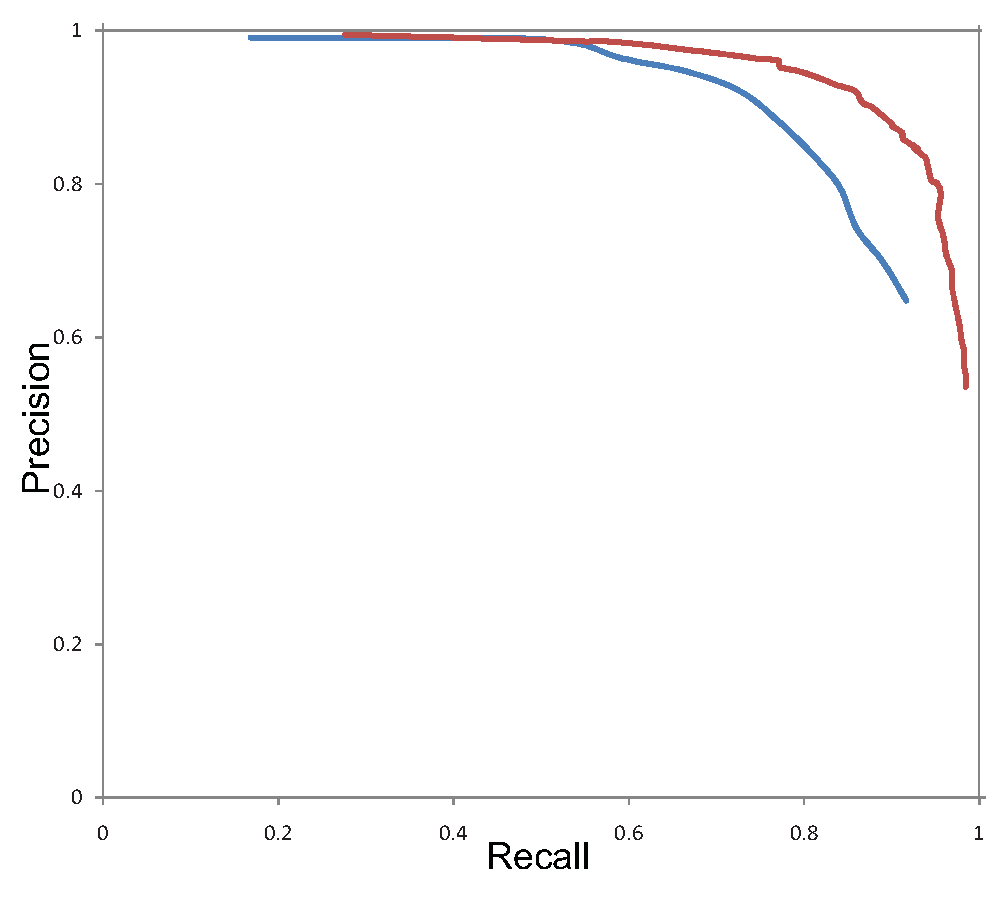
\includegraphics[width=0.23\textwidth,bb=0 0 480 425]{prf.eps}
\label{fig:pr:a}}
\subfigure[]{
\begin{minipage}[b]{0.22\textwidth}
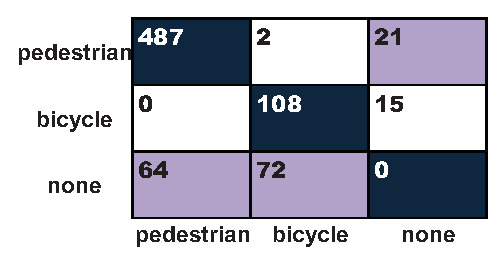
\includegraphics[width=\textwidth,bb=0 0 230 115]{cm2.eps}\\
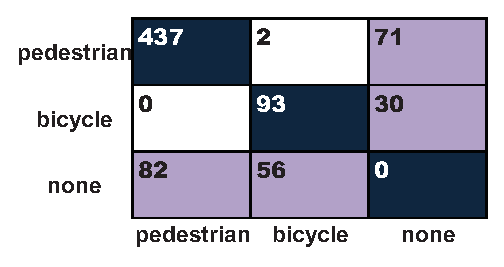
\includegraphics[width=\textwidth,bb=0 0 230 115]{cm1.eps}
\end{minipage}
\label{fig:pr:b}}
\caption{Precision-recall curves (red: the proposed method, blue: the benchmark method) and confusion matrices (upper: the proposed method, down: the benchmark method). In (b), pedestrian and bicycle miss detections are considered as wrongly recognized to be none. Pedestrian or bicycle false alarms are considered as belonging to the none class while wrongly recognized as pedestrians or bicycles.}
\label{fig:pr}
\end{figure}

The precision-recall curves are shown in Figure \ref{fig:pr:a}. An object is considered as correctly detected only if the distance from the ground truth to it is less than 10 pixels. In Figure \ref{fig:pr:a}, the correctly detected but wrongly recognized objects are considered as true positives, aiming at verifying the detection ability of the proposed method.

The confusion matrices are given in Figure \ref{fig:pr:b}. For clarity of the comparisons, the proposed method is compared with the benchmark method when they have nearly equal number of false alarms. To evaluate the concurrent detection and recognition ability, a class of {\lq\lq}none{\rq\rq} to represent missed detections and false alarms is manually added. For example, in Figure \ref{fig:pr:b}, 487 pedestrian instances are correctly detected and recognized by the proposed method, 2 are wrongly recognized to be bicycle riders, and 21 are miss-detected.

\begin{figure*}
\centering
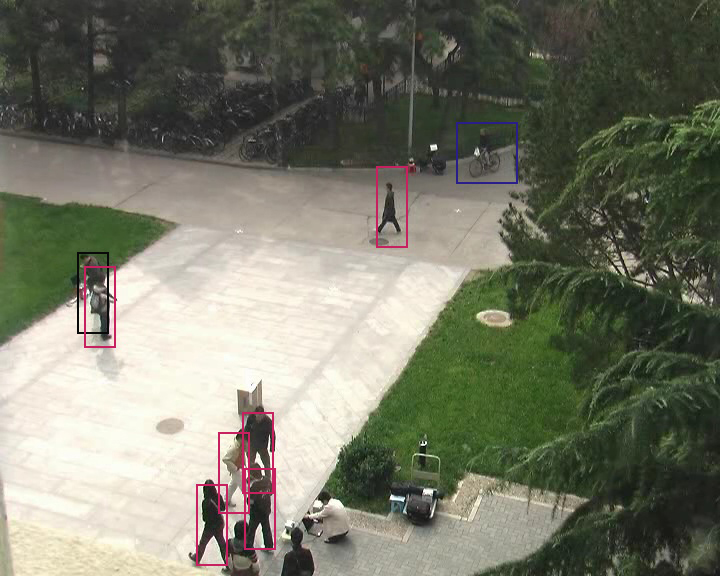
\includegraphics[width=0.23\textwidth,bb=0 0 720 576]{016.jpg}
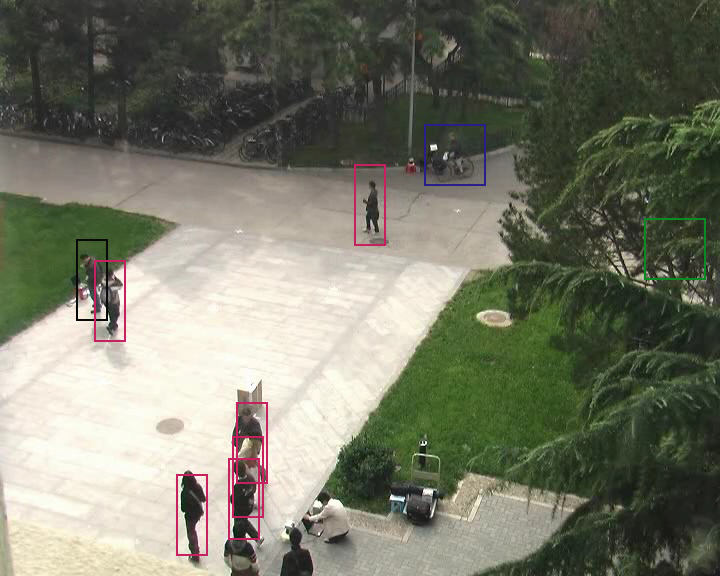
\includegraphics[width=0.23\textwidth,bb=0 0 720 576]{026.jpg}
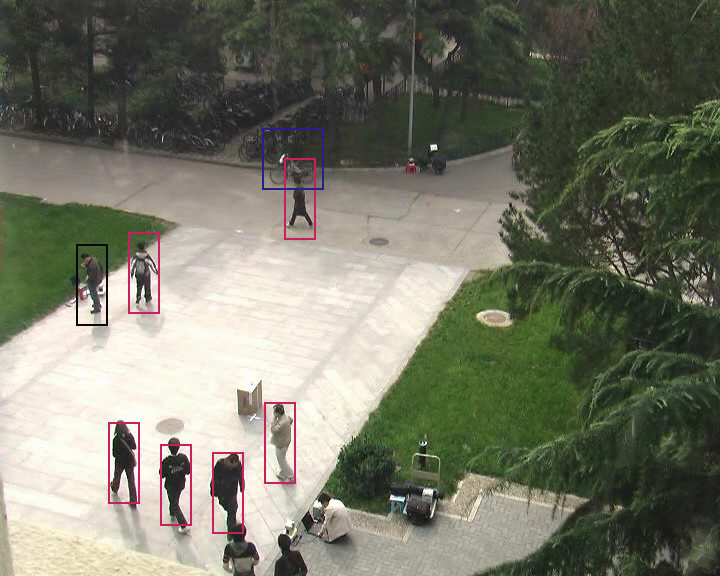
\includegraphics[width=0.23\textwidth,bb=0 0 720 576]{071.jpg}
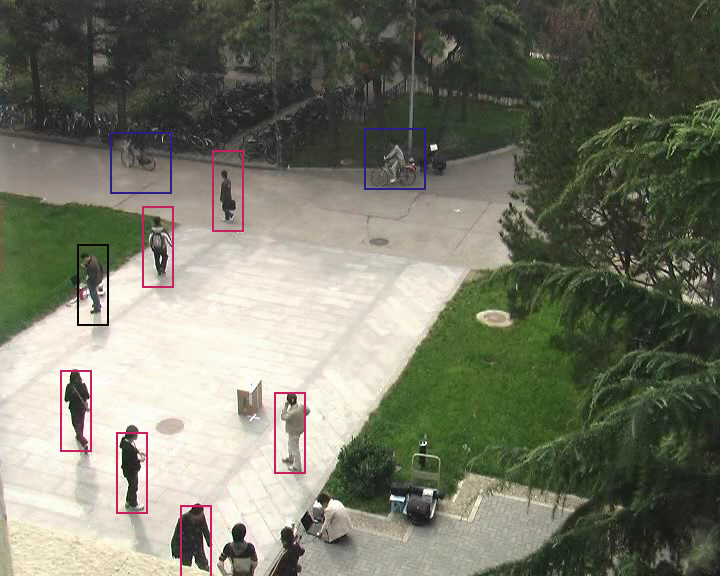
\includegraphics[width=0.23\textwidth,bb=0 0 720 576]{116.jpg}


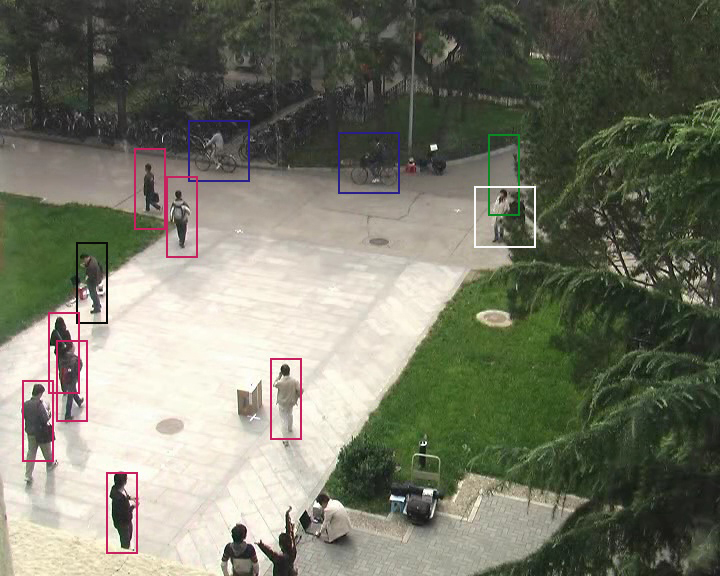
\includegraphics[width=0.23\textwidth,bb=0 0 720 576]{166.jpg}
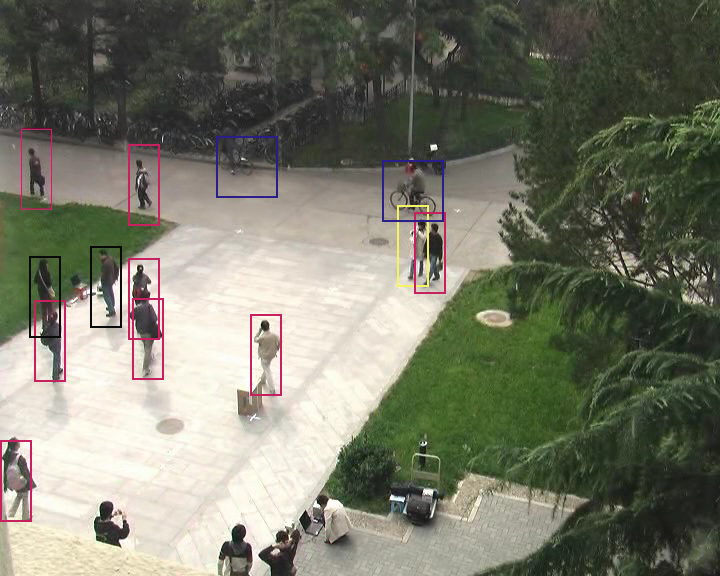
\includegraphics[width=0.23\textwidth,bb=0 0 720 576]{251.jpg}
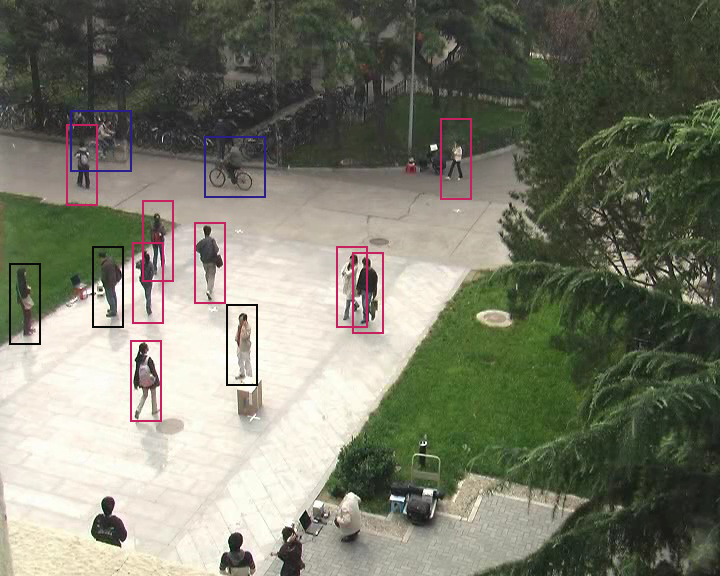
\includegraphics[width=0.23\textwidth,bb=0 0 720 576]{326.jpg}
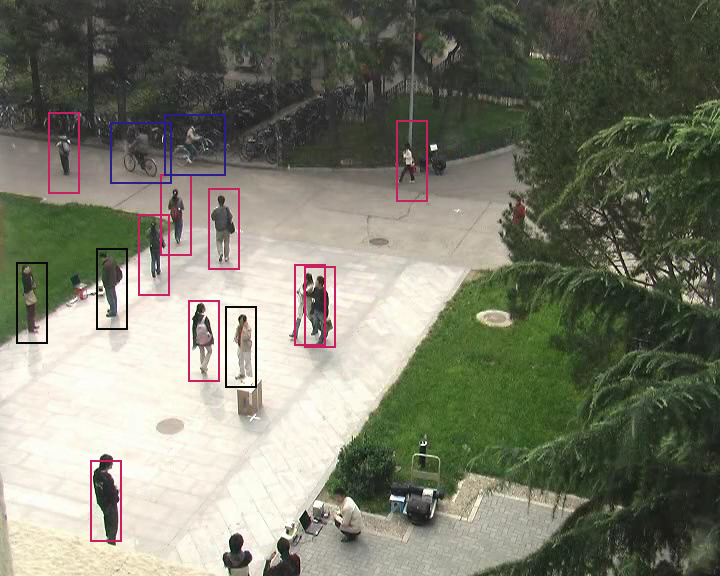
\includegraphics[width=0.23\textwidth,bb=0 0 720 576]{366.jpg}
\caption{Campus objects detection and recognition results. Red rectangles and blue rectangles mark correctly detected and recognized pedestrians and bicycle riders. Yellow rectangles mark missed detections. White rectangles mark correctly detected but not correctly recognized objects. Green rectangles mark false alarms. Black rectangles mark static objects, which are beyond the verification for the method.}
\label{fig:result}
\end{figure*}

The proposed method is limited by its relying on reliable motion information. As shown in Figure \ref{fig:result}, failures occur when objects enter the scene.

\subsection{Big {\lq\lq}{Cats}{\rq\rq} Detection and Recognition}

\begin{figure}
\centering
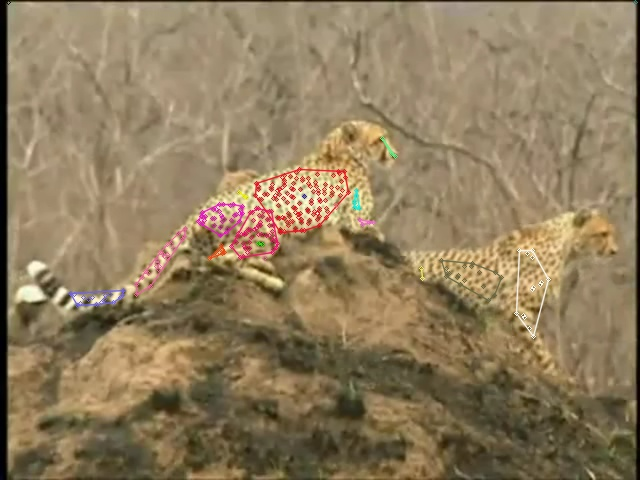
\includegraphics[width=0.23\textwidth,bb=0 0 640 480]{amotionimg00296.jpg}
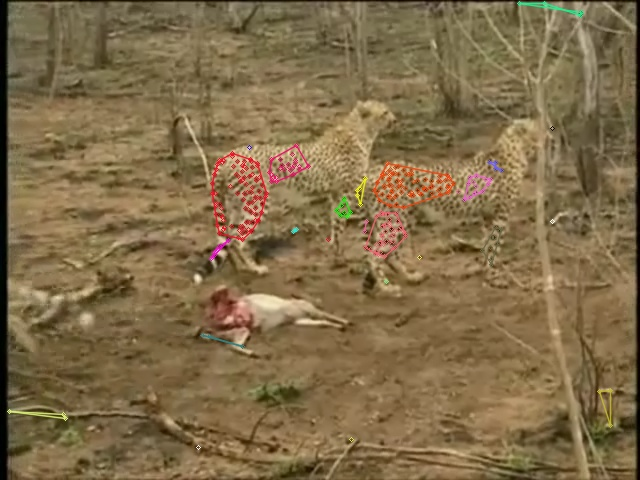
\includegraphics[width=0.23\textwidth,bb=0 0 640 480]{amotionimg01836.jpg}

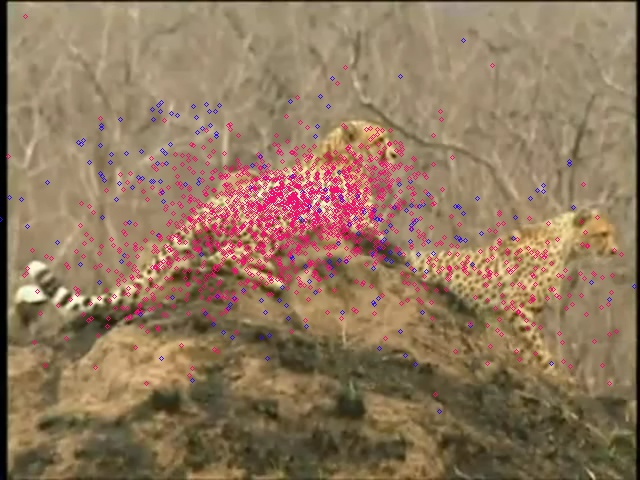
\includegraphics[width=0.23\textwidth,bb=0 0 640 480]{selectVimg00296_0.jpg}
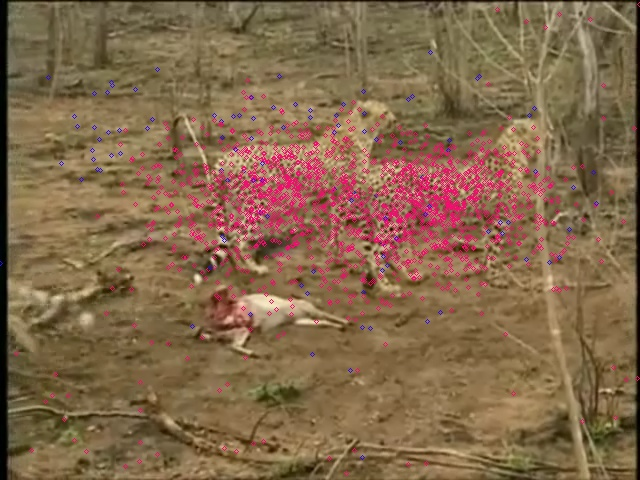
\includegraphics[width=0.23\textwidth,bb=0 0 640 480]{selectVimg01836_0.jpg}

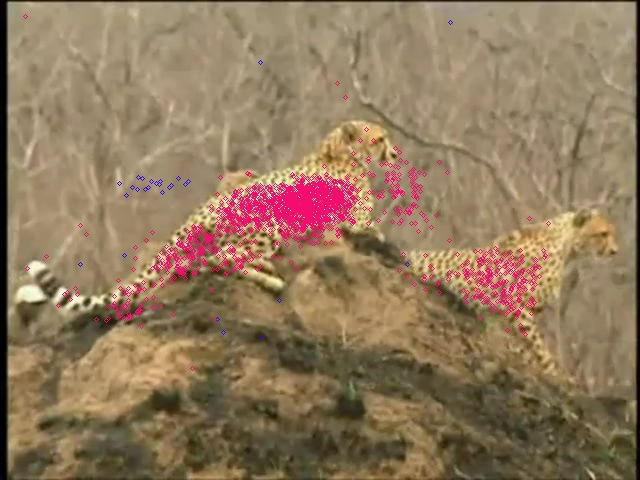
\includegraphics[width=0.23\textwidth,bb=0 0 640 480]{selectVimg00296_19.jpg}
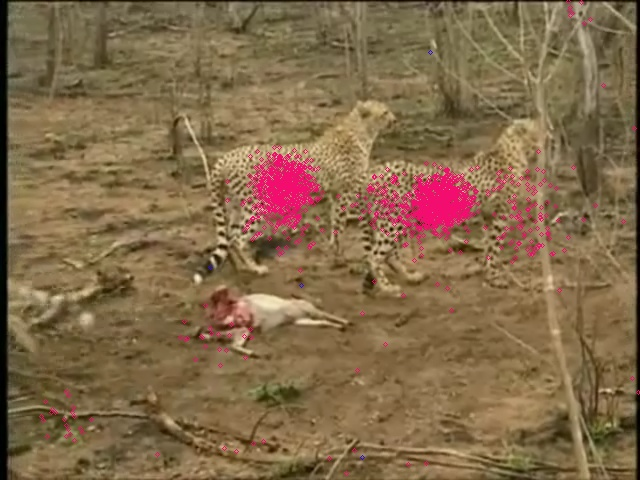
\includegraphics[width=0.23\textwidth,bb=0 0 640 480]{selectVimg01836_19.jpg}

\caption{Effect of the proposed prior. Red circles are voted center for leopards, while blue ones are voted centers for tigers. On the top are the motion grouping results. In the middle are the voted centers according to the best matched codes. On the bottom are the voted centers voted by votes with highest priors.}
\label{fig:bcMP}
\end{figure}

\begin{figure}
\centering


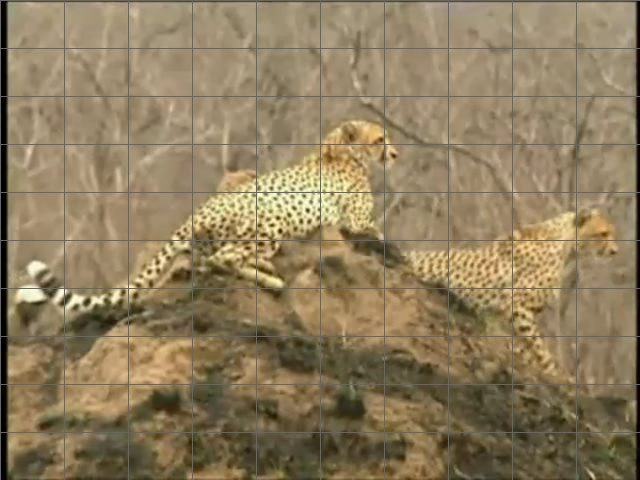
\includegraphics[width=0.23\textwidth,bb=0 0 640 480]{PER1.jpg}
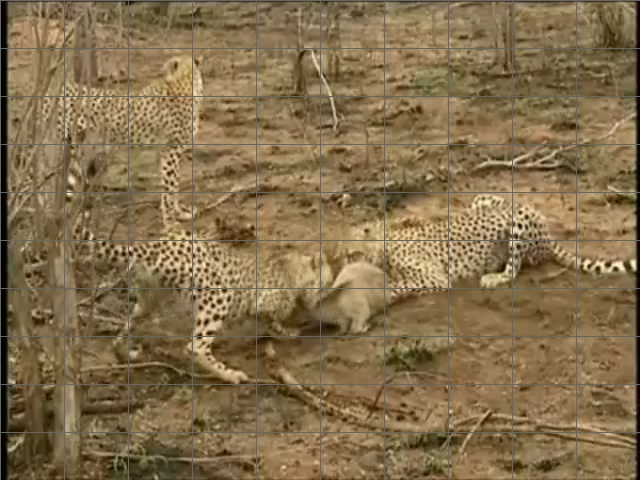
\includegraphics[width=0.23\textwidth,bb=0 0 640 480]{PER2.jpg}

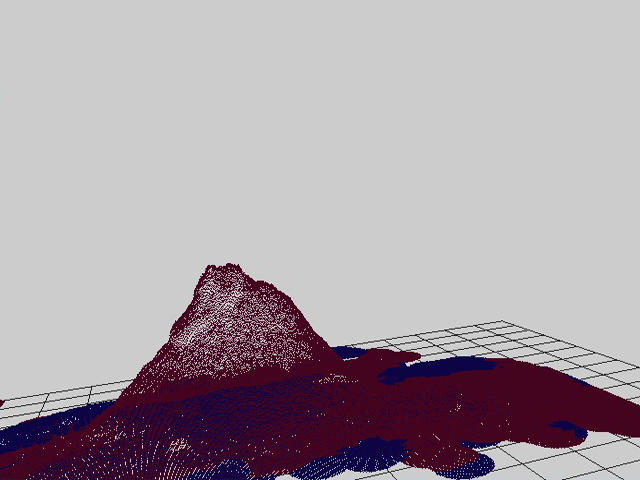
\includegraphics[width=0.23\textwidth,bb=0 0 640 480]{1.jpg}
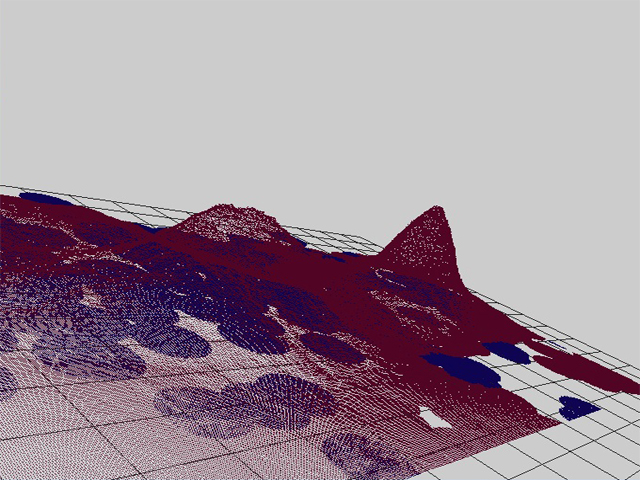
\includegraphics[width=0.23\textwidth,bb=0 0 640 480]{3.jpg}

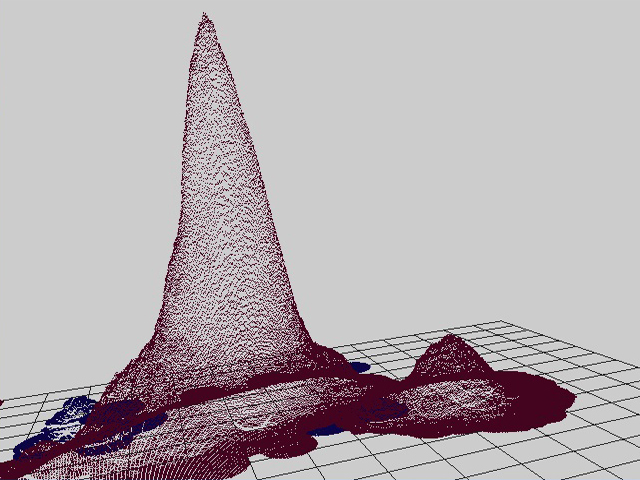
\includegraphics[width=0.23\textwidth,bb=0 0 640 480]{2.jpg}
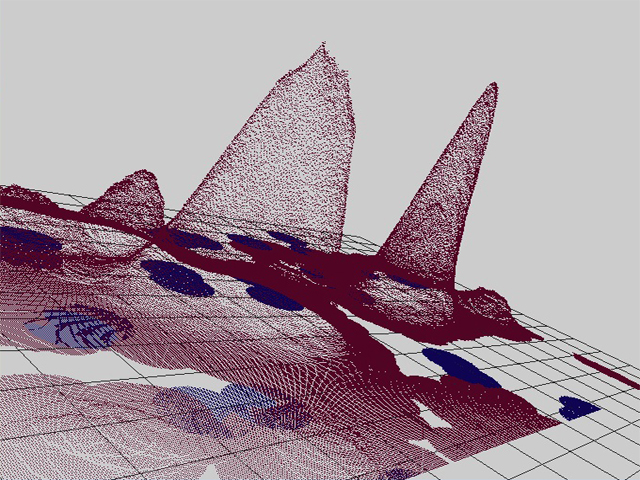
\includegraphics[width=0.23\textwidth,bb=0 0 640 480]{4.jpg}


\caption{Example Hough images. On the top are the original images. In the middle are the Hough images formed by votes with uniform priors. On the bottom are the Hough images formed by votes with the proposed priors. Red indicates leopards, and blue indicates tigers. Note for the two leopards, there is no peak corresponding to the right one on the benchmark Hough image. For the three leopards, there is also no peak corresponding to the leopard in behind on the benchmark Hough image.}
\label{fig:BcHi}
\end{figure}
\textbf{Dataset} To further verify the proposed method, a mini dataset is built upon leopards and tigers of the family Felidae. The dataset contains 6 video clips of 9 leopards and 4 tigers. The frame size is 640$\times$480. Both the animals are in the side view.

\textbf{Implementation settings} Most implementation settings are the same with the settings for campus object detection and recognition. For training, 5 leopards and 2 tigers are used. The size of the image patch around each keypoint is 27$\times$27.




\textbf{Comparisons} In Figure \ref{fig:bcMP}, the motion grouping results and how the voted centers are affected are given. Since parts from different positions of the leopard are very similar, the true center of a leopard is difficult to find from the voted centers of the object parts. In Figure \ref{fig:BcHi}, example Hough images are given to show the merit of the proposed prior by the ability to detect leopards. In Figure \ref{fig:bgdr}, the detection and recognition results are given. The proposed method successfully detects and recognizes all the leopards and tigers, while the benchmark method miss-detects three leopards.

\begin{figure}
\centering
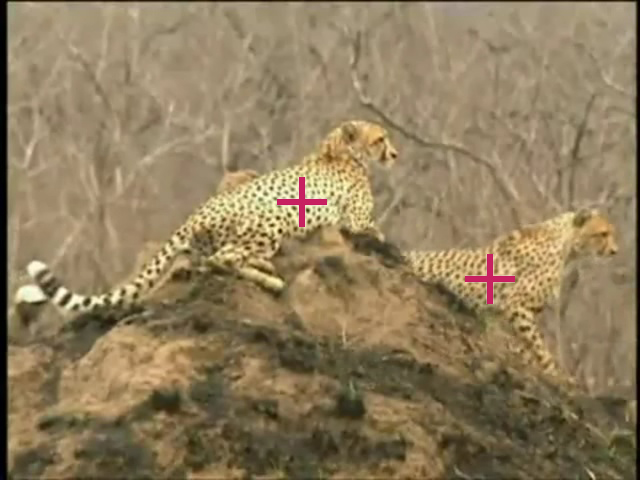
\includegraphics[width=0.23\textwidth,bb=0 0 640 480]{leo1.jpg}
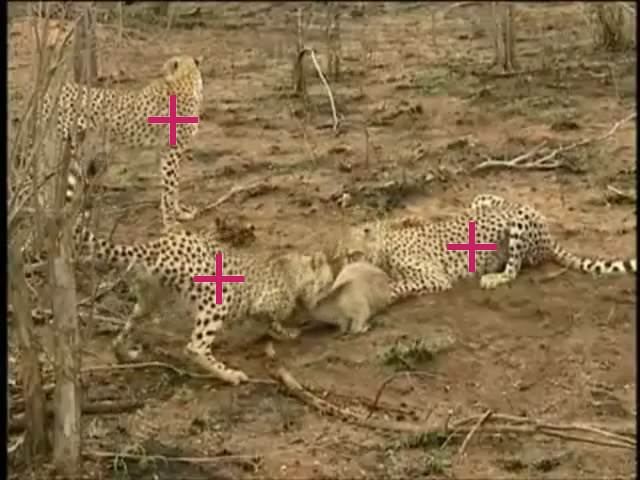
\includegraphics[width=0.23\textwidth,bb=0 0 640 480]{leo2.jpg}

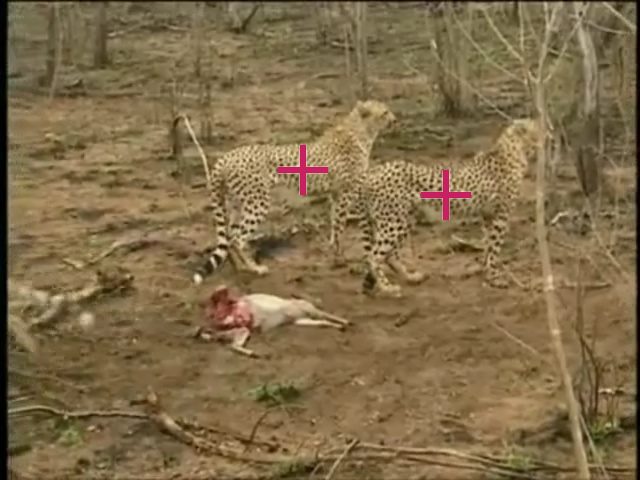
\includegraphics[width=0.23\textwidth,bb=0 0 640 480]{leo3.jpg}
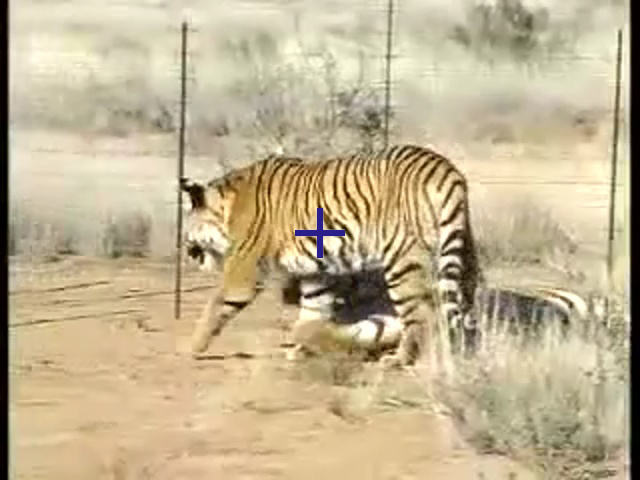
\includegraphics[width=0.23\textwidth,bb=0 0 640 480]{ti1.jpg}

\caption{Big {\lq\lq}{cats}{\rq\rq} detection and recognition results. Red crosses mark the centers for leopards and blue crosses mark the centers for tigers.}
\label{fig:bgdr}
\end{figure}

\section{Discussion and Conclusion}
This paper proposes a method for concurrent detection and recognition by extending the probabilistic Hough transform with motion. The underlying assumption is that object parts moving coherently are likely to belong to the same object. Before voting, all the object parts are grouped by their motion patterns. The votes of each object part are given different priors according to the motion grouping results. In this manner, the proposed method enhances the traceability of the Hough image formed. Experiments show the merit of the method in terms of detection and recognition accuracy.




{\small
\bibliographystyle{ieee}
\bibliography{egbib}
}


\end{document}
